\documentclass[a4paper]{paper}

%----------------����ctex�����֧������
\usepackage[left=1.25in,top=1.25in,right=1.25in,bottom=1.25in,head=1.25in]{geometry}
\usepackage{setspace}
\usepackage{geometry}
\usepackage{indentfirst}
\usepackage{float}
\usepackage{hyperref}
\usepackage{fancyhdr}
\usepackage{graphicx}

%-----------------ҳüҳ������
\pagestyle{fancy}
\lhead{}
\chead{Cancel or not? Predictive Analysis for Hotel Booking Data}
\rhead{}
\lfoot{}
\cfoot{\thepage}
\rfoot{}
\renewcommand{\headrulewidth}{1pt}
\renewcommand{\footrulewidth}{0pt}


\setlength{\parindent}{2em}
\renewcommand{\baselinestretch}{1.2}

\title{\textbf{Cancel or not?\\Predictive Analysis for Hotel Booking Data}}
\author{\normalsize{Jingwei Gao, Simon SHEN, Yingjie Jiang, Rongxin Ouyang}}
\date{}


\begin{document}
	
	\maketitle

	
	\section{Project description}
	
	Emerging network society issues new challenges on understanding big data in electronic consuming behaviors, as well as in hotel business. Significant differences can be easily found in tremendous reservation records, consisting of time, location, historic characteristics, etc., however, the utilization of hotel booking data can be conducive to optimizing business decisions and strategies but also far from application without quantified nuances behind the topsoils.
	
	In order to explore, disentangle, and predict cancellation behavior, we initialized this project based on a recent and popular dataset on kaggle:
	
	\begin{table}[H]
		\centering
		\caption{\textbf{Project description}}\label{tab:01}
		\begin{tabular}{l|p{10cm}l}
			\hline
			\textbf{Project} & \textbf{Details} \\ \hline
			Goal & To predict whether a specific hotel booking will be cancelled. \\ \hline
			Data & \href{https://www.kaggle.com/jessemostipak/hotel-booking-demand}{Kaggle link: Hotel booking demand}\\ \hline
			Data File & hotel\_bookings.csv \\ \hline
			Data Description & This data set contains booking information for a city hotel and a resort hotel, and includes information such as when the booking was made, length of stay, the number of adults, children, and/or babies, and the number of available parking spaces, among other things. \\ \hline
		\end{tabular}
	\end{table}
	
	\section{Task, significance and process}
	
	\subsection{Project task}
	
	This project is proposed to use order information of multiple dimensions order to predict whether a specific order will be cancelled or not.

	\subsection{Significance}
	
	Before the user cancels the order, it is predicted whether the user will cancel the order, which is beneficial to the hotel and the reservation website to better allocate resources, improve the true utilization rate of resources, and maximize the revenue. The problem of overselling airline tickets by analog airlines, overselling airline tickets within a reasonable range, helps to achieve a balance between customer efficiency and company revenue, and achieves the most profit without harming the customer experience.

	\subsection{Process}
	
	\textbf{Determine the data set.} There are a lot of open source data on kaggle, considering the significance of the topic and the difficulty of prediction, and finally select the hotel prediction topic.
	
	\textbf{Identify the problem.} Taking into account the hotel booking time, whether to cancel the order is of great significance to the hotel or the user. At the same time, the cancellation of the predetermined behavior and other variables in the data set have a causal relationship, so we determine the research direction to determine whether the user cancels the order.
	
	\textbf{Data exploration.} Correlation analysis of data and feature engineering processing of data sets using pca method.
	
	\textbf{Classical model (tree based).} In this section, initially, we'll start with two classical baseline models, logistic regression and randomforest with default parameter, and then use boosting techniques to improve the performance of tree-based models in two efficient modern frameworks, LightGBM and XGBoost.
	
	\textbf{Deep learning model.} Although we have derived a nice result (i.e. high accuracy) from gradient boosting algorithms, we still want to know how the deep learning model performs in this task. We choose to use a simple feed-forward neural network as our deep learning model. We fix the network structure in advance and do some hyperparameter tuning to find whether it is possible to get a better result. At last, we use LIME to approximate a local explanation for our DL model.

	\section{Data exploration}
	
	Exploration on the meanings of features was conducted before formal exploratory analysis.
	
	\subsection{Feature with meaning}
	
	Please refer to the appendix A for further details of this part.

	\subsection{Correlations and PCA}
	
	With the help of our \underline{\href{https://github.com/oyrx/PHBS_MLF_2019_Project/blob/master/code/Corrleations_And_Feature_Engineering.ipynb}{manual work}} and \underline{\href{https://github.com/oyrx/PHBS_MLF_2019_Project/blob/master/code/Exploration_Statistics.ipynb}{pandas\_profiling}}, we discern that:
	
	\textbf{Cramer's V model}: Cramer's V model based on the chi squared statistic that can show how strongly nominal variables are associated with one another. This is very similar to correlation coefficient where 0 means no linear correlation and 1 means strong linear correlation.
	
	- Drop some features: As we did before, two features ("reservation\_status\_date" \& "reservation\_status") are dropped for avoidance of leakage. In addition, we drop the feature "arrival\_date\_year" because we will use future information to predict future cancellation behavior.
	
	- Results: "deposit\_type" showed the highest correlation with the target variable. The reservation\_status\_date effect was already looked at in the previous section where we saw an intersting trend that people cancel less during the winter time.
	
	\textbf{Numerical features's correlations}
	
	- Drop some features: re-convert "is\_canceled" attribute to numerical values.
	- Results: both lead\_time and total\_of\_special\_requests had the strongest linear correlations with is\_canceled target variable.
	
	\textbf{PCA analysis on categorical features}
	
	- OneHotEncoding: To convert categorical features to numerical ones using Scikit-learn. This requires running integer encoding first followed by OneHotEncoding.
	
	- Results: the principal component 1 holds 44.2\% of the information while the principal component 2 holds only 32.9\% of the information. Summing them up, we will have ~77\% of information. We need about 8 components to represent 90\% of the dataset.
	Other details of each feature can be found at \href{https://github.com/oyrx/PHBS_MLF_2019_Project/blob/master/docs/Descriptive_Report.html}{descriptive report}.
	
	\section{Data cleaning}
	
	Target variable in this study is is\_canceled (0/1) and features are available from 31 different dimensions. Among them, all 30 dimensions are discrete variables, and only adr (Average Daily Rate) is a continuous variable.
	
	Thanks to preliminary data cleaning by the owner of data, only a small amount of vacant values need to be filled. More specifically, the data cleaning procedure includes:
	
	- Fill the na value of the children factor. Considering that the children and babies factor have a small difference and the vacancy values of the children field are very few, they are filled directly with the babie field.
	
	- The other fields with vacant values are all categorical fields. Here we want to retain as many features as possible, so fill in the vacant values as 'undefined' and do not delete them.

	\section{Baseline and tree-based models}
	
	This section contains two baseline models, LR and Random Forest, and other two moder boosting methods, Dart in LightGBM and GBDT in XGBoost.
	
	\subsection{Methodology}
	
	\vspace{5pt}
	
	\noindent \textbf{What is GBDT and DART?}
	
	Gradient Boosted Decision Trees (GBDT) is a machine learning algorithm that iteratively constructs an ensemble of weak decision tree learners through boosting.
	
	For GBDT: 1) Feature selection is inherently performed during the learning process. 2) Not prone to collinear/identical features. 3) Models are relatively easy to interpret. 4) Easy to specify different loss functions.
	
	For DART: Similar to GBDT but \underline{\href{https://lightgbm.readthedocs.io/en/latest/Parameters-Tuning.html}{may be more accurate than GBDT}}.\vspace{-5pt}\\
	
	\noindent \textbf{Why LightGBM and XGBoost?}
	
	\textit{Why do we deliberately use those two similar, to some extend, boosting framework?} The first reason is that DART, a slightly different method, is also comprised in LightGBM, which would provide diversity for our potential model candidates. Second, XGBoost and LightGBM use discrepent tree growth strategies ( level-wise vs. leaf-wise) and the difference should not been ignored in finding the best hyper-parameters, especially when that level-wise leads to unexpected ramifications like over-fitting is literally a commonplace for professional data-scientists.
	
	We're curious about the nuances between level-wise tree growth and leaf-wise tree growth, thus, we decide to run both LightGBM and XGBoost.
	
	Implementation and tuning are similar to LightGBM though caterical features in numeric way is acceptable in XGBoost.
	
	\begin{figure}[ht]
		\centering
		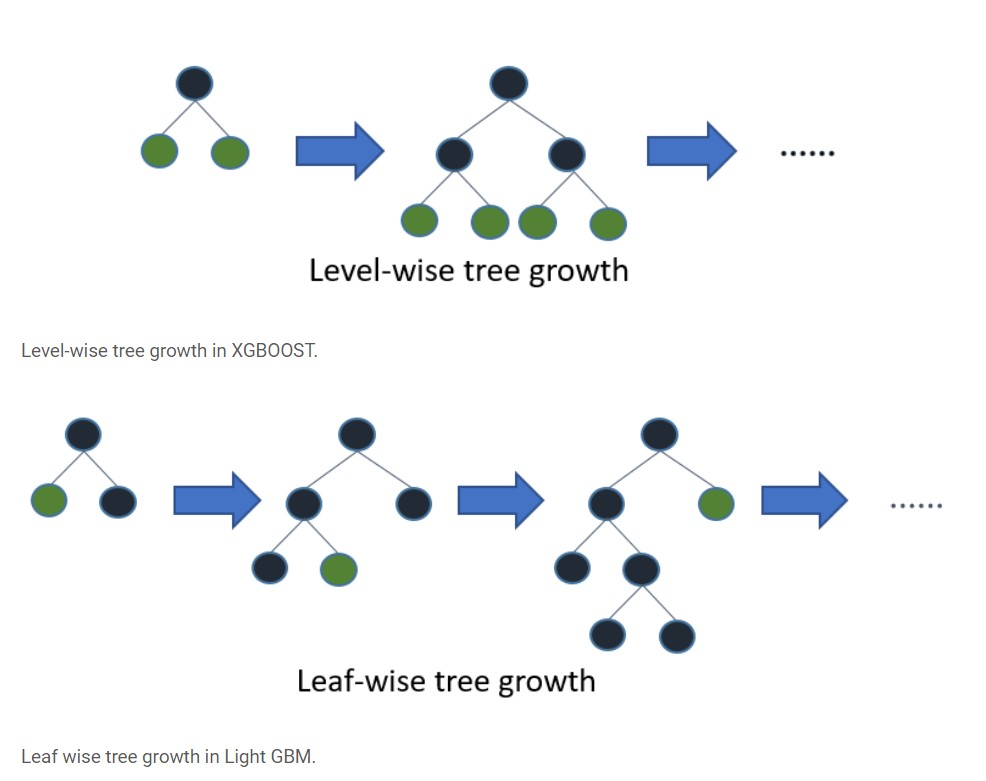
\includegraphics[scale=0.4]{01.jpg}
		\caption{Leaf wise tree growth in LightGBM}
		\label{fig:tu1}
	\end{figure}

	\subsection{Preparation}
	
	Based on previously cleaned and splitted datasets, consistent standarization and some extra process were carried out to fit model requirements.
	
	A fairly significat issue here is datatype. According to the design and implementation of LightGBM, categorical features \underline{\href{https://lightgbm.readthedocs.io/en/latest/Advanced-Topics.html}{should be kept in interger}}, thereby, the process of standarization was divided into two different chunks to relinquish categorial features and then bring them back.
	
	Incidentally, for engineering convinience, we also introduced a redesigned function named "algorithm\_pipeline()" to expedite implementation through predefined datasets, fit criteria, and reusable grid search process.

	\begin{figure}[ht]
		\centering
		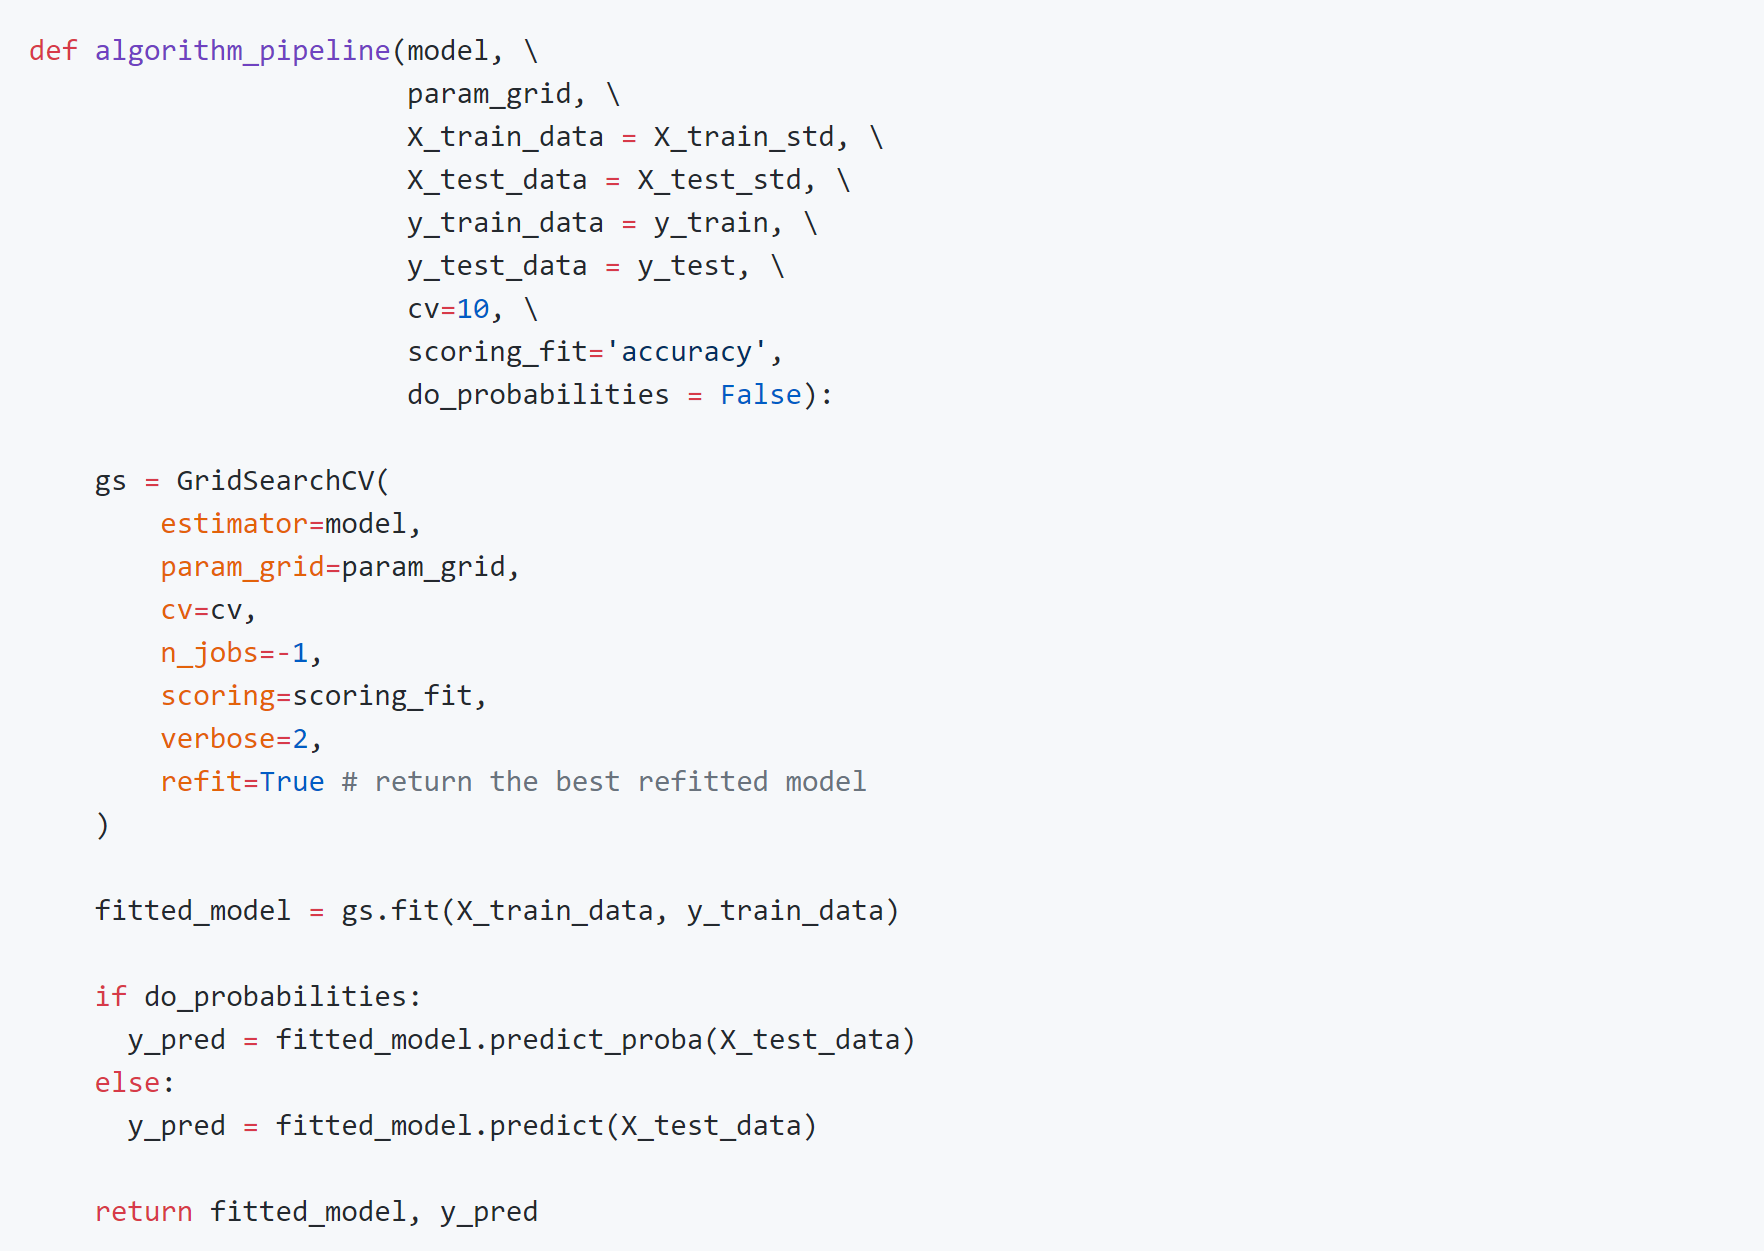
\includegraphics[scale=0.5]{02.png}
		\caption{algorithm pipeline}
		\label{fig:tu2}
	\end{figure}

	\subsection{Models}
	
	\subsubsection{Baseline: Logistic Regression and Random Forest}
	
	Starting with two baseline models, a logistic regression with l2 regularization and a random forest model with limited n\_estimators, we find that a simple logistic regression is literally ��not bad�� as an approximately 80\% accuracy on the testing set and random forest performs much better, scoring at 89\%.
	
	However, random forest is very slow for training a single model even with highly constrained n\_estimators. Heeding the advice from Jingwei Gao, we decide to acquaint the application of two modern boosting framework, XGBoost and LightGBM to accelerate parameter tuning process and improve the ability of generalization.

	\subsubsection{DART in LightGBM and GBDT in XGBoost}
	
	With the help of scaffolding, those two modules and one customized grid search function, a lot of combinations of hyperparameters are efficiently tested according to the manuscript in official docementation in following process:
	
	- First, experiments were conducted to find a generally optimized parameter dict of num\_leaves, min\_data\_in\_leaf and max\_depth.
	
	- Second, tuning other paramters to get higher accuracy in both training data and testing data, where slightly over-fitting on testing set is accpetable.
	
	- Then, apply regularization and other constraints and other constraints to tackle over-fitting.
	
	- In order to improve computational performance, sub-sampling and limited cross validation folds are consecutively applied in the whole process.
	
	\begin{figure}[ht]
		\centering
		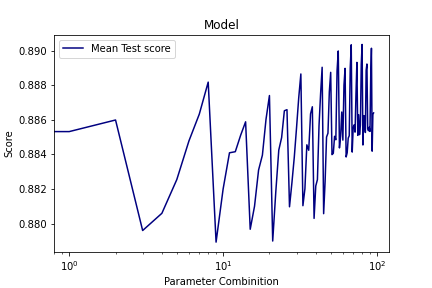
\includegraphics[scale=0.7]{03.png}
		\caption{LightGBM cvresult\protect\footnotemark[1]}
		\label{fig:tu3}
	\end{figure}\footnotetext[1]{Parameters ange were selected on previous training results and not continouous due to limited computation capacity}

	Eventually, a modern modelwith boosting techniques, DART in LightGBN, takes the crown with testing accuracy up to 89.61\%.
	
	\subsection{Result}
	
	\subsubsection{Results in short}
	
	1) A DART(LightGBM) Model with accuracy upto approximately 90\%(89.61\%).
	
	2) Manifold predominant features: lead\_time, adr(Average Daily Rate, dividing the sum of all lodging transactions by the total number of staying nights), arrival\_date\_day\_of\_month, arrival\_date\_week\_number, country, agent, etc., representing characteristics of time, place, actor, laws of normal transactions, and so on.
	
	3) Relatively easy-to-interpretant tree model
	
	\subsubsection{Results in detail}
	
	\vspace{-5pt}
	
	\begin{table}[H]
		\centering
		\caption{\textbf{Model Comparison}}\label{tab:02}
		\begin{tabular}{p{2.7cm}p{2cm}p{2cm}p{3cm}p{2.5cm}}
			\hline
			& \textbf{LogReg} & \textbf{RF} & \textbf{LGBM(DART)} & \textbf{XGB(GBDT)} \\ \hline
			Accuracy (Train) & 0.79377 & 0.97796 & 0.98896 & 0.99574 \\ \hline
			Accuracy (Test) & 0.79433 & 0.8925 & 0.89614 & 0.89404 \\ \hline
			Precision & 0.80 & 0.89 & 0.90 & 0.89 \\ \hline
			Recall & 0.79 & 0.89 & 0.90 & 0.89 \\ \hline
			F1-score & 0.79 & 0.89 & 0.90 & 0.89 \\ \hline
		\end{tabular}
	\end{table}

	\vspace{-5pt}
	
	\begin{table}[H]
		\centering
		\caption{\textbf{Hyperparameters Optimization Results}}\label{tab:02}
		\begin{tabular}{p{3cm}p{10cm}}
			\hline
			\textbf{Model} & \textbf{Parameters} \\ \hline
			Logistic Regression & \{'boosting': 'DART', 'feature\_fraction': 0.7, 'lambda\_l2': 0.1, 'max\_depth': 25, 'min\_split\_gain': 0.1, 'n\_estimators': 3000, 'num\_leaves': 100, 'objective': 'binary'\} \\ \hline
			Random Forest & \{'n\_estimators': '100', 'max\_depth': 25, 'random\_state' : 0, 'bootstrap': True\} \\ \hline
			LightGBM(DART) & \{'boosting': 'DART', 'feature\_fraction': 0.7, 'lambda\_l2': 0.1, 'max\_depth': 25, 'min\_split\_gain': 0.1, 'n\_estimators': 3000, 'num\_leaves': 100, 'objective': 'binary'\} \\ \hline
			XGBoost(GBDT) & \{'colsample\_bytree': 0.7, 'max\_depth': 50, 'n\_estimators': 100, 'reg\_alpha': 1.3, 'reg\_lambda': 1.1, 'subsample': 0.9\} \\ \hline
		\end{tabular}
	\end{table}
	\vspace{-13pt}
	\noindent \small{\textit{* Abbr. for Gradient Boosted Decision Trees}}\\
	\noindent \small{\textit{* Small n\_estimators in Random Forest on purpose.}}


	\begin{table}[H]
		\centering
		\caption{\textbf{Best Model: Confusion Matrix}}\label{tab:02}
		\begin{tabular}{lllll}
			\hline
			\textbf{Value} & \textbf{precision} & \textbf{recall} & \textbf{f1-score} & \textbf{support} \\ \hline
			0 & 0.91 & 0.93 & 0.92 & 15033 \\ \hline
			1 & 0.88 & 0.84 & 0.86 & 8845 \\ \hline
			\textbf{General} &  &  &  &  \\ \hline
			accuracy & - & - & 0.90 & 23878 \\ \hline
			macro avg & 0.89 & 0.88 & 0.89 & 23878 \\ \hline
			weighted avg & 0.90 & 0.90 & 0.90 & 23878 \\ \hline
		\end{tabular}
	\end{table}
	\vspace{-13pt}
	\noindent \small{\textit{* Train(accuracy): 98.896\%}}\\
	\noindent \small{\textit{* Test(accuracy): 89.614\%}}

	\begin{figure}[ht]
		\centering
		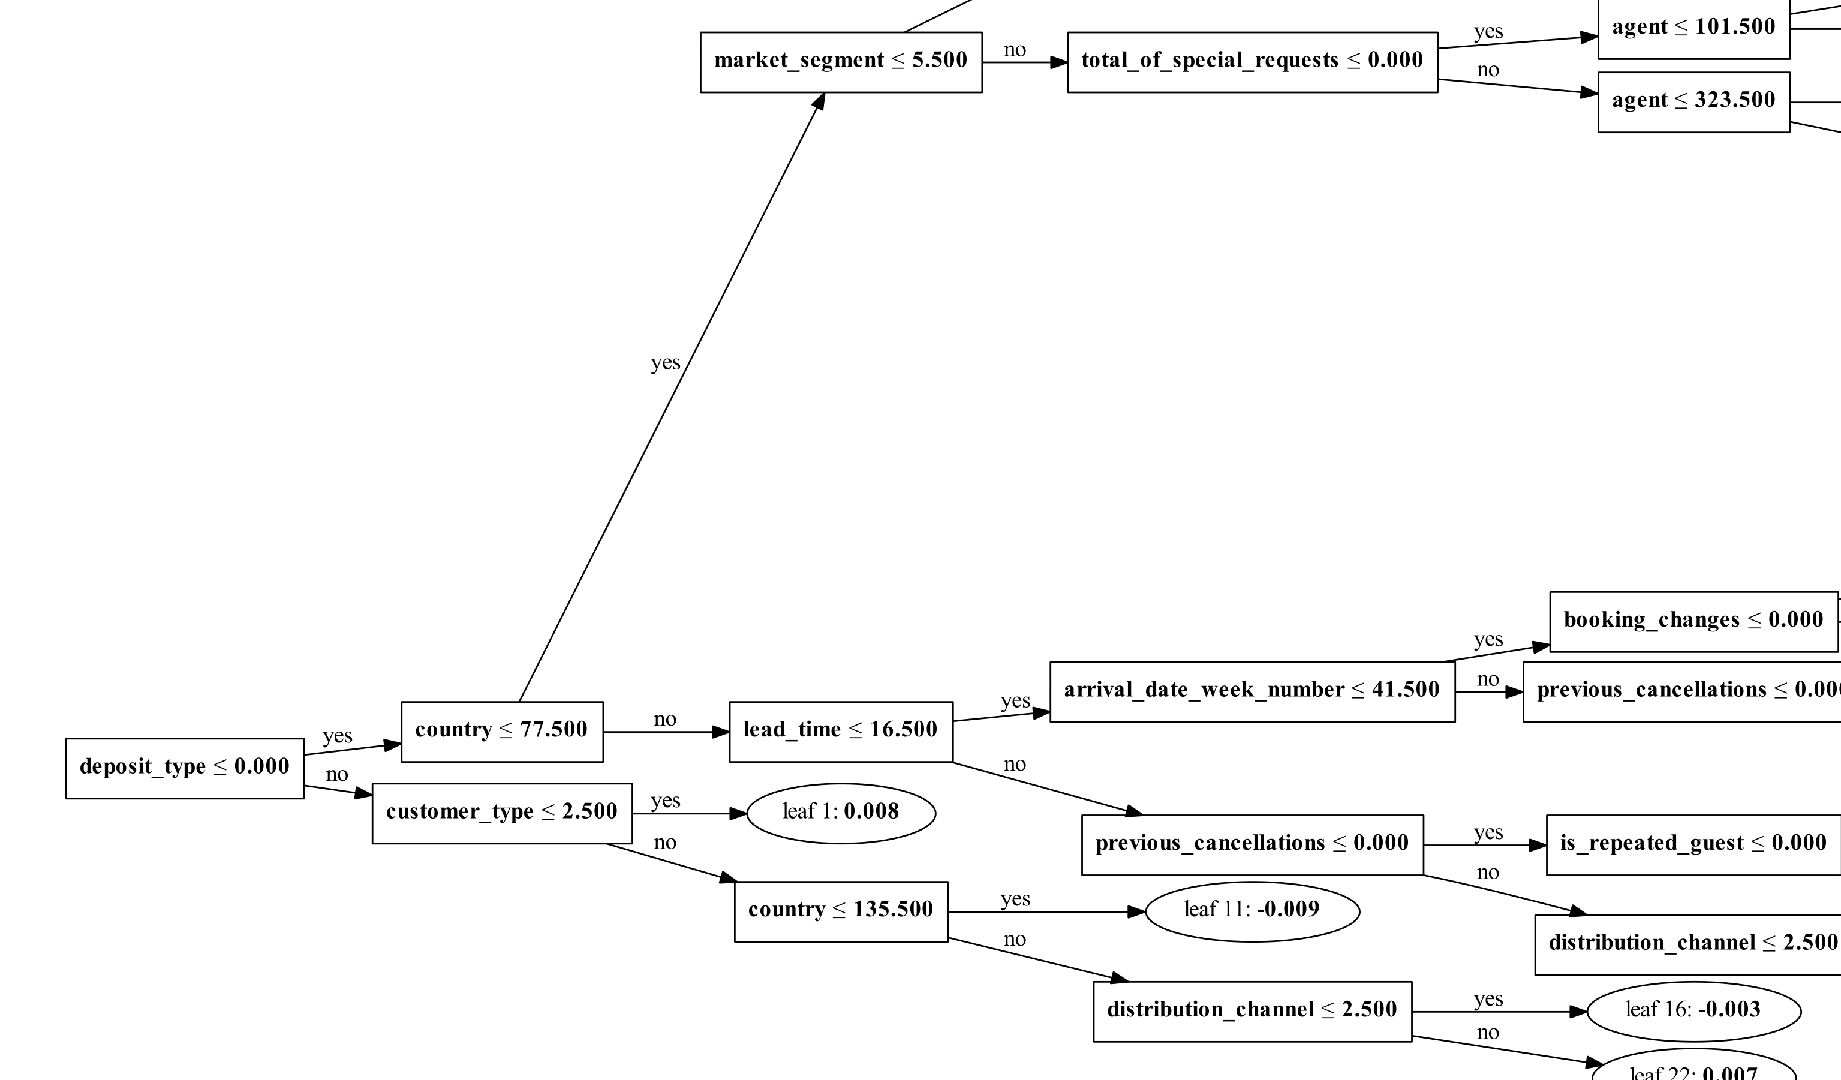
\includegraphics[scale=0.3]{04.png}
		\caption{Best Model: Tree Plot\protect\footnotemark[2]}
		\label{fig:tu4}
	\end{figure}\footnotetext[2]{See: \href{https://github.com/oyrx/PHBS_MLF_2019_Project/raw/master/images/LighGBM.png}{\underline{full tree}}}
			 
			
	\begin{figure}[ht]
		\centering
		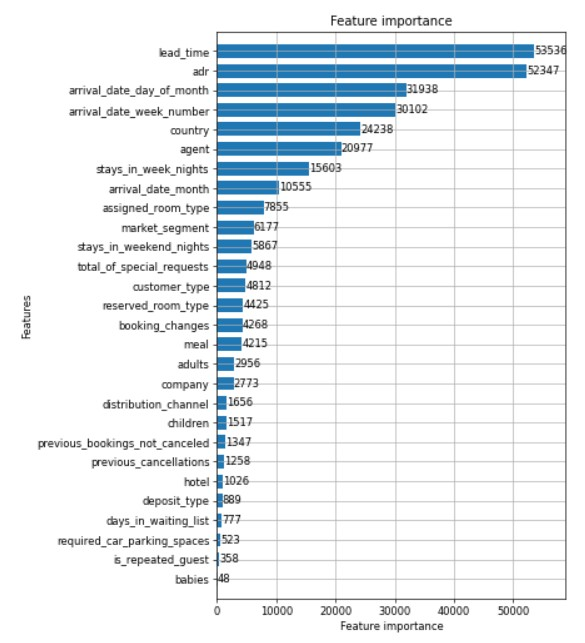
\includegraphics[scale=0.6]{05.jpg}
		\caption{Best Model: Feature Importance}
		\label{fig:tu5}
	\end{figure}

	\section{Deep learning model\protect\footnotemark[3]}
	
	\footnotetext[3]{\href{https://drive.google.com/file/d/1tcqmtkpZdIR0qgnDTeY34Mlj11_x--q-/view?usp=sharing}{\underline{Colab - Notebook - All codes}}}
	
	Although we have derived a beautiful result (i.e. high accuracy) from gradient boosting algorithms, we still want to know how the deep learning model performs in this task. Because there is little information about time series in this data set, we choose to use a simple feed-forward neural network as our deep learning model.
	
	\subsection{Toolkit: PyTorch}
	
	PyTorch is an open source machine learning library and is widely used in deep learning scenarios for its flexibility. PyTorch uses dynamic computational graphs rather than static graphs, which can be regarded as the mean difference between it and other deep learning frameworks. To get more information on PyTorch, click here.
	
	\begin{figure}[ht]
		\centering
		
\includegraphics[scale=0.05]{06.png}
		\caption{PyTorch}
		\label{fig:tu6}
	\end{figure}

	\subsection{Data preprocessing}
	
	\textbf{Drop some features}: As we did before, two features ("reservation\_status\_date" \& "reservation\_status") are dropped for avoidance of leakage. In addition, we drop the feature "arrival\_date\_year" because we will use future information to predict future cancellation behavior. We drop the feature "arrival\_date\_month" because we can get it from the combination of "arrival\_date\_week\_number" and "arrival\_date\_day\_of\_month".
	
	\textbf{One-hot encodin}g: One-hot encoder is used to convert categorical data into integer data. Since there are many categories under "company" and "agent", data's dimension increases to 1025 after the one-hot encoding.
	
	\textbf{Validation se}t: We use 20\% data in \textit{train.csv} as our validation data. Batch size: 6000.

	\subsection{Network structure}

	\begin{figure}[ht]
		\centering
		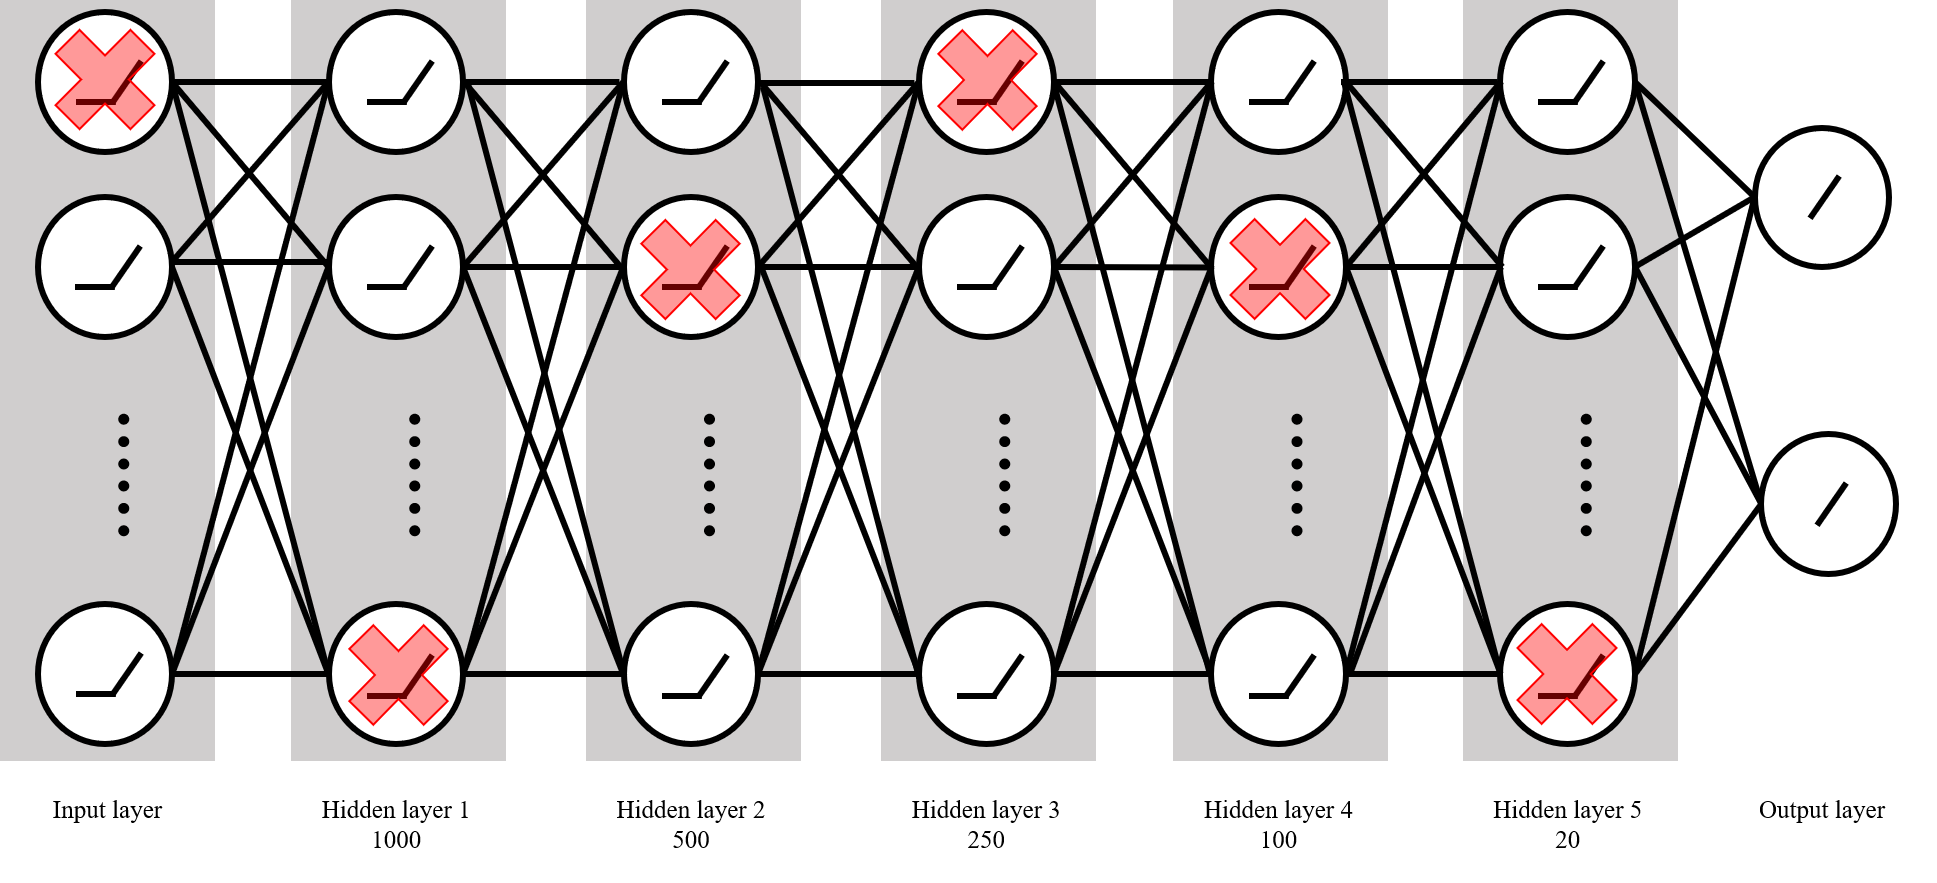
\includegraphics[scale=0.3]{07.png}
		\caption{Network structure}
		\label{fig:tu7}
	\end{figure}

	1)Input$\rightarrow$1000$\rightarrow$500$\rightarrow$250$\rightarrow$100$\rightarrow$20$\rightarrow$2
	
	2)Dropout before doing batch normalization
	
	3)Choose Sigmoid/Tanh/ReLU as activation function

	\subsection{Hyperparameter tuning}
	
	It is a binary classification task, so we use cross-entropy as our loss function and apply early stopping to avoid over-fitting. Because we use dropout as a tool of regularization, we need to determine the dropout rate dr. We use Adam as adaptive learning rate method and fix $\beta_1$ and $\beta_2$ by using their default values, but we still need to determine the learning rate lr. At last, we want to compare the average performance of three kinds of activation function (sigmoid, Tanh, ReLU). Hence, there are three kinds of parameters that need to be tuned:
	
	1) learning rate lr for Adam: [0.005, 0.05]
	
	2) dropout rate dr: [0.2, 0.8]
	
	3) activation function: sigmoid, tanh, ReLU
	
	We use random search rather than grid search for hyperparameter tuning ���� Randomly select 120 parameter combinations. The result is as follows:
	
	\begin{figure}[ht]
		\centering
		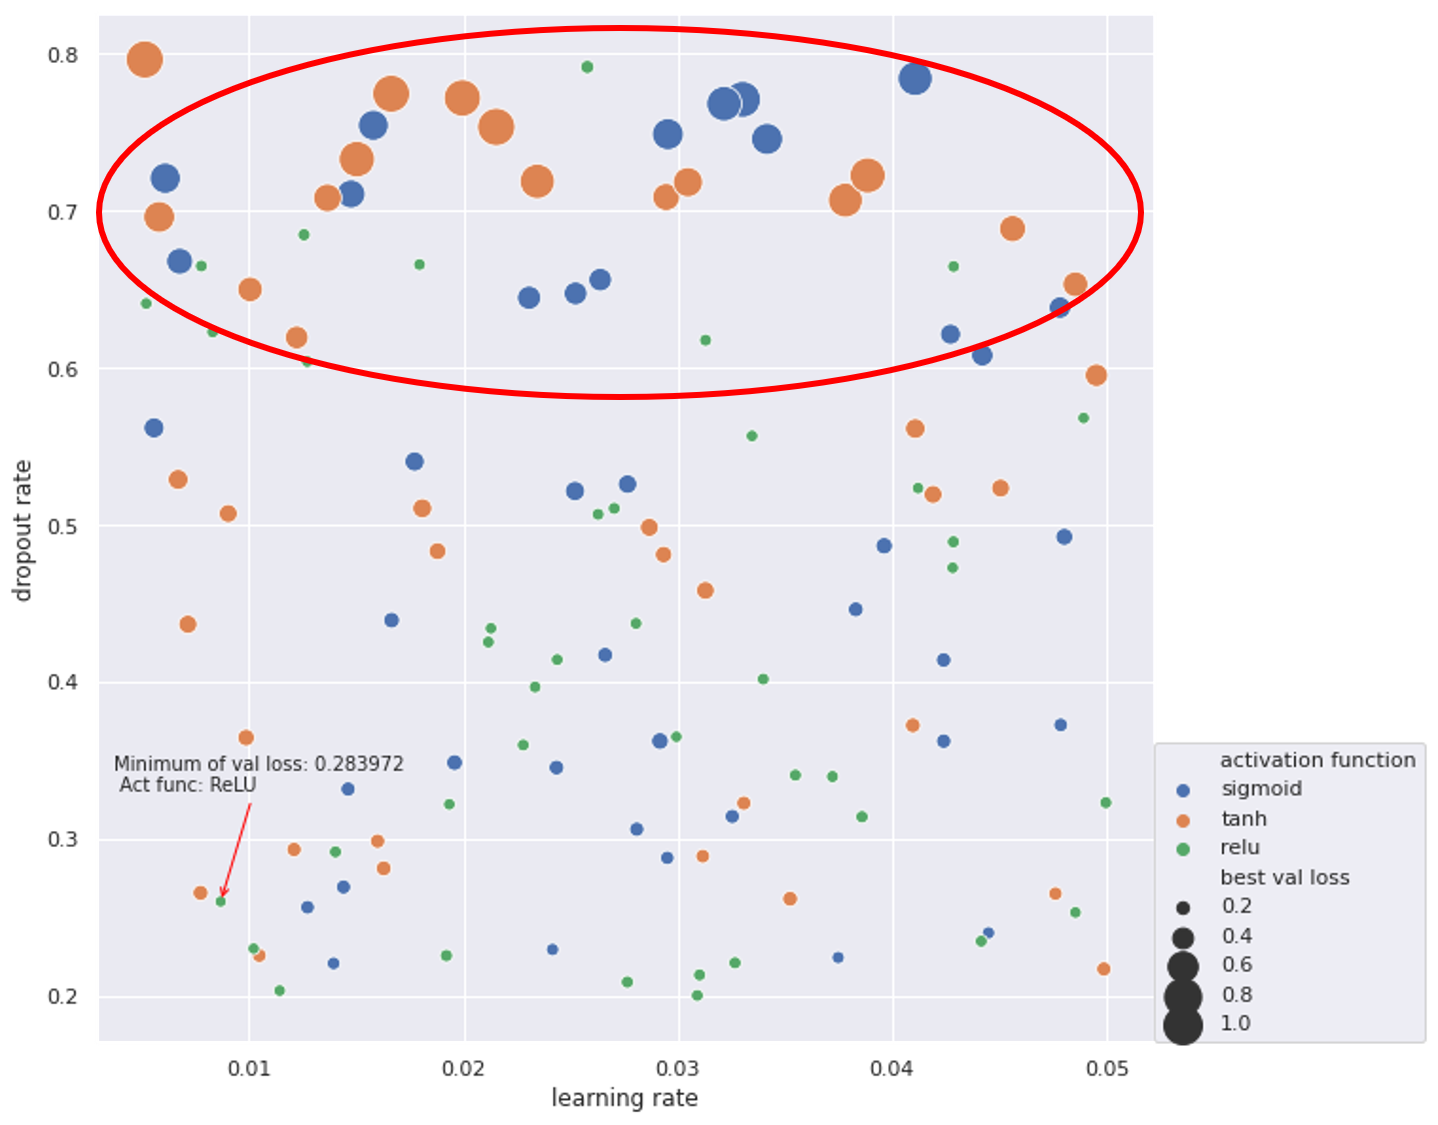
\includegraphics[scale=0.6]{08.png}
		\caption{Result of random search}
		\label{fig:tu8}
	\end{figure}

	\noindent The best parameters among these 120 combinations are:
	
	1) learning rate: 0.00867688
	
	2) dropout rate: 0.260069
	
	3) activation function: ReLU
	
	The corresponding validation loss is 0.283972. The validation accuracy is 0.870927. From the scatterplot, we can see that ReLU is a better choice for activation function because of its stableness. When dropout rate is high (0.6~0.8), using sigmoid or tanh as activation function will get bad results ($loss \approx 1.0$). However, ReLU can still provide a small loss and high accuracy in that region.

	\subsection{Retrain \& Test}
	
	At last, we use the hyperparameters from the last step and retrain the model on the whole training data (original training set + validation set). The learning process:
	
	\begin{figure}[ht]
		\centering
		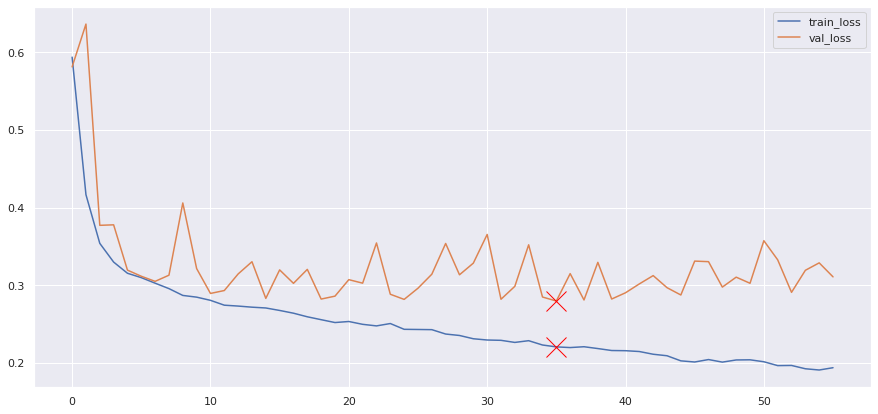
\includegraphics[scale=0.4]{09.png}
		\caption{Retrain \& test}
		\label{fig:tu9}
	\end{figure}

	The test loss is about 0.280 and test accuracy is about 0.875. Other performance metrics on test set:
	
	\begin{table}[H]
		\centering
		\caption{\textbf{Final DL model}}\label{tab:05}
		\begin{tabular}{lllll}
			\hline
			\textbf{Value} & \textbf{precision} & \textbf{recall} & \textbf{f1-score} & \textbf{support} \\ \hline
			0 & 0.88 & 0.92 & 0.90 & 15033 \\ \hline
			1 & 0.85 & 0.78 & 0.82 & 8845 \\ \hline
			\textbf{General} &  &  &  &  \\ \hline
			accuracy & - & - & 0.87 & 23878 \\ \hline
			macro avg & 0.87 & 0.85 & 0.86 & 23878 \\ \hline
			weighted avg & 0.87 & 0.87 & 0.87 & 23878 \\ \hline
		\end{tabular}
	\end{table}
	
	\subsection{Explainable deep learning model}
	
	At last, we want to make this deep learning model explainable in some sense. So we try to apply LIME (\href{https://arxiv.org/pdf/1606.05386.pdf}{\underline{Local Interpretable Model-agnostic Explanations}}) on the model we trained above in order to get some hints from the local explanation.
	
	1) First, we notice that DL model predicts the 21st test instance as [label 1] with probability distribution [0.00001, 0.99999]. We choose this data point as our "local point".
	
	2) Second, we sample 5000 instances nearby. In particular, we fix the value of categorical variables and only do sampling in terms of numerical variables for convenience.
	
	3) Use DL model to predict the labels of these 5000 sample. After that ,we get 5000 new "training data".
	
	4) We choose logisitic regression as the simple model to explain the DL model locally ���� Train the LR model on 5000 new "training data" in order to mimic the DL model's behavior locally. The accuracy is 98.86\%.
	
	5) Finally, we get the coefficients before the numerical variables. It is worth noting that the coefficient before "previous\_cancellations" is +6.31 and the coefficient before "required\_car\_parking\_spaces" is -13.9. This result shows the judgment logic of the DL model: \textbf{people who have cancelled the order before have a higher probability of canceling this order and people who reserved parking spaces are less likely to cancel this order}.

	\begin{figure}[ht]
		\centering
		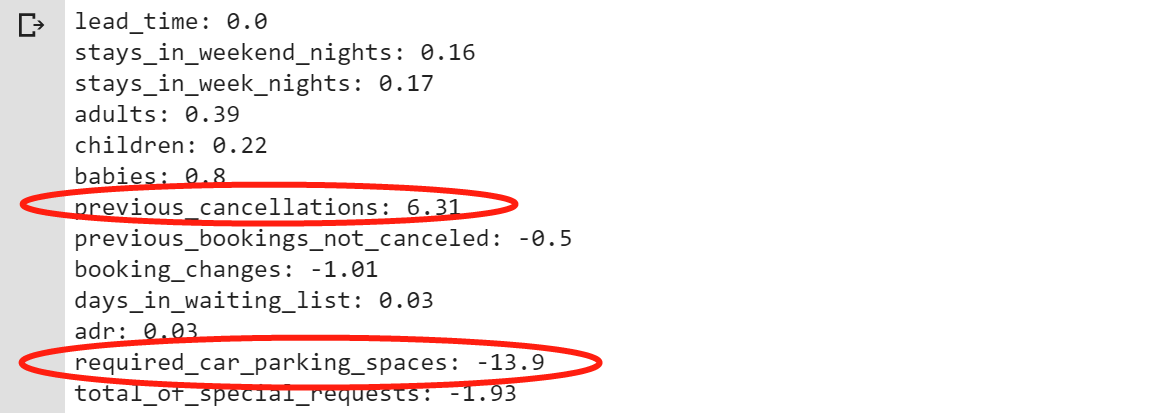
\includegraphics[scale=0.7]{10.png}
		\caption{Coefficients in LR model}
		\label{fig:tu10}
	\end{figure}

	\subsection{Summary}
	
	Results from multifold models, including traditional ML techniques and DL strategies, indicate the failure of deep learning model to defeat the gradient boosting methods. This unanticipated ramification can be ascribed to the following reasons.
	
	\textbf{Misplaced advantages}: It's commonplace that a deep learning model is more efficient dealing with unstructured data such as images and text by extracting meaningful representations. However, all the data here is highly structured, which creates convenience for conventional models.
	
	\textbf{Parameter dilemma}: Deep learning models need to adjust more parameters in order to get better results in such context. Among all the hyperparameters, network structure is quite important, however, due to limited computation capacity the network structure has to be fixed in advance. That's to say, a trap of network structure has impeded our progress at the very beginning.
	
	\section{Conclusions}
	
	This project uses several machine learning models to predict reservation cancellation. Among them, DART in LightGBM beats other competitors with highest testing accuracy (table) and also other metrics.
	
	\begin{table}[H]
		\centering
		\caption{\textbf{Test accuracy}}\label{tab:06}
		\begin{tabular}{llllll}
			\hline
			 & LogReg & RF & LightGBM (DART) & XGBoost (GBDT) & ANN \\ \hline
			Test Accuracy & 0.79433 & 0.8925 & 0.89614 & 0.89404 & 0.875\\ \hline
		\end{tabular}
	\end{table}

	Results from our models also tally our supposition that time, place, actor, laws of normal transactions are killers in predicting such behaviors (lead\_time, adr, arrival\_date\_day\_of\_month, arrival\_date\_week
	\_number, country, agent).
	
	Correspondingly, cancellation issue a hotel may face can be duly tackled by accelerating or rectifying business strategies using our effective and interpretable model.
	
	Learning from the practice and comparison of conventional machine learning models and a slightly overkilling deep learning technique (ANN), we may conclude our experience as: \textbf{"Deep" is not always the "Jeep"}.
	
\end{document}